\chapter{Moti relativi}
Si consideri un corpo puntiforme $P$ in movimento lungo una generica traiettoria. Il suo moto viene osservato da un sistema di riferimento con centro $O$, che per convezione si chiama fisso, e da un secondo sistema di riferimento con centro $O'$ di coordinate $O'\equiv(x_0,y_0,z_0)$ rispetto ad $O$, che per convezione si chiama mobile. L'origine del sistema mobile ha una velocità $v_{O'}$ rispetto al sistema fisso, inoltre l'insieme dei tre assi in generale ruota rigidamente con velocità angolare $\omega$. L'obiettivo è determinare quali sono le relazioni tra la posizione, la velocità e l'accelerazione del punto $P$, misurate da un osservatore solidale con il sistema fisso, e le corrispondenti grandezze misurate da un osservatore solidale con il sistema mobile. La relazione tra le posizioni del punto $P$, misurate rispetto ai due sistemi di riferimento, è
\begin{equation}
    \vr=\vr_{O'}+\vri,
\end{equation}
dove
\begin{equation}
    \begin{cases}
        \vr=x\hatu_x+y\hatu_y+z\hatu_z \\
        \vr_{O'}=x_0\hatu_x+y_0\hatu_y+z_0\hatu_z \\
        \vri=x'\hatu_{x'}+y'\hatu_{y'}+z'\hatu_{z'} \\
    \end{cases}.
\end{equation}
Quindi, le velocità $\vv$, $\vvi_r$ e $\vv_{O'}$ sono
\begin{equation}
    \begin{split}
        \vv&=\frac{d\vr}{dt}=\frac{d}{dt}(x\hatu_x+y\hatu_y+z\hatu_z) \\
        &=\frac{dx}{dt}\hatu_x+\frac{dy}{dt}\hatu_y+\frac{dz}{dt}\hatu_z+x\frac{d\hatu_x}{dt}+y\frac{d\hatu_y}{dt}+z\frac{d\hatu_z}{dt}\\
        &=\frac{dx}{dt}\hatu_x+\frac{dy}{dt}\hatu_y+\frac{dz}{dt}\hatu_z,
    \end{split}
\end{equation}
\begin{equation}
    \begin{split}
        \vv_{O'}&=\frac{d\vr_O'}{dt}=\frac{d}{dt}(x_0\hatu_x+y_0\hatu_y+z_0\hatu_z) \\
        &=\frac{dx_0}{dt}\hatu_x+\frac{dy_0}{dt}\hatu_y+\frac{dz_0}{dt}\hatu_z+x_0\frac{d\hatu_x}{dt}+y_0\frac{d\hatu_y}{dt}+z_0\frac{d\hatu_z}{dt} \\
        &=\frac{dx_0}{dt}\hatu_x+\frac{dy_0}{dt}\hatu_y+\frac{dz_0}{dt}\hatu_z,
    \end{split}   
\end{equation}
e
\begin{equation}
    \begin{split}
        \vvi_r&=\frac{d\vri}{dt}=\frac{d}{dt}(\xp\hatu_\xp+\yi\hatu_\yi+\zi\hatu_\zi) \\
        &=\frac{d\xp}{dt}\hatu_\xp+\frac{d\yi}{dt}\hatu_\yi+\frac{d\zi}{dt}\hatu_\zi+\xp\frac{d\hatu_\xp}{dt}+\yi\frac{d\hatu_\yi}{dt}+\zi\frac{d\hatu_\zi}{dt},
    \end{split}
\end{equation}
dove si è usato il fatto che $\hatu_x$, $\hatu_y$ e $\hatu_z$ hanno modulo e direzione costante. Usando $\vr=\vr_{O'}+\vri$, la velocità $\vv$ diventa
\begin{equation}
    \begin{split}
        \vv&=\frac{d}{dt}(\vr_{O'}+\vri)=\frac{d\vr_{O}}{dt}+\frac{d\vri}{dt} \\
        &=\frac{dx_0}{dt}\hatu_x+\frac{dy_0}{dt}\hatu_y+\frac{dz_0}{dt}\hatu_z+ \\
        &+\frac{d\xp}{dt}\hatu_\xp+\frac{d\yi}{dt}\hatu_\yi+\frac{d\zi}{dt}\hatu_\zi+\xp\frac{d\hatu_\xp}{dt}+\yi\frac{d\hatu_\yi}{dt}+\zi\frac{d\hatu_\zi}{dt} \\
        &=\vv_{O'}+\vvi+(\xp\vom\times\hatu_\xp+\yi\vom\times\hatu_\yi+\zi\vom\times\hatu_\zi) \\
        &=\vv_{O'}+\vvi+\vom\times(\xp\hatu_\xp+\yi\hatu_\yi+\zi\hatu_\zi) \\
        &=\vv_{O'}+\vvi+\vom\times\vri.
    \end{split}
\end{equation}
La velocità $\vvi$ non è altro che la velocità del punto $P$ rispetto al sistema di riferimento mobile. Dunque, la relazione tra la velocità osservata nel sistema di riferimento fisso $\vv$ e quella osservata nel sistema di riferimento mobile $\vvi$ è data dal teorema delle velocità relative
\begin{equation}
\label{eq: teorema delle velocità relative}
    \vv=\vvi+\vv_{O'}+\vom\times\vri.
\end{equation}
Il termine correttivo $\vv_t=\vv-\vvi=\vv_{O'}+\vom\times\vri$ è detto velocità di trascinamento e dipende dai parametri del sistema di riferimento mobile e dalla posizione del punto $P$ rispetto a tale sistema: corrisponde alla velocità assoluta di un punto solidale con il sistema mobile. Si presentano due casi base:
\begin{enumerate}
    \item Se il sistema mobile non ruota rispetto a quello fisso, ossia $\vom=0$, allora l'equazione \eqref{eq: teorema delle velocità relative} diventa $\vv=\vvi+\vv_{O'}$. In questo caso si parla di moto di trascinamento traslatorio.
    \item Se il sistema mobile non si muove rispetto a quello fisso, ossia $\vv_{O'}$, allora l'equazione \eqref{eq: teorema delle velocità relative} diventa $\vv=\vvi+\vom\times\vri$. In questo caso si parla di moto di trascinamento rotatorio.
\end{enumerate}
Il caso generale può essere pensato come somma di un moto relativo traslatorio e uno rotatorio tra i due sistemi. 

Partendo da $\eqref{eq: teorema delle velocità relative}$ si può ricavare una relazione analoga tra le accelerazioni osservate nei due sistemi di riferimento. Quindi, le accelerazioni $\va$, $\vai_r$ e $\va_{O'}$ sono
\begin{equation}
    \begin{split}
        \va&=\frac{d\vv}{dt}=\frac{d}{dt}\bigg(\frac{dx}{dt}\hatu_x+\frac{dy}{dt}\hatu_y+\frac{dz}{dt}\hatu_z\bigg)=\frac{d^2x}{dt^2}\hatu_x+\frac{d^2y}{dt^2}\hatu_y+\frac{d^2z}{dt^2}\hatu_z,
    \end{split}
\end{equation}
\begin{equation}
    \va_{O'}=\frac{d\vv_{O'}}{dt  }=\frac{d^2x_0}{dt^2}\hatu_x+\frac{d^2y_0}{dt^2}\hatu_y+\frac{d^2z_0}{dt^2}\hatu_z,
\end{equation}
\begin{equation}
    \begin{split}
        \vai_r&=\frac{d\vvi_r}{dt}=\frac{d}{dt}\bigg(\frac{d\xp}{dt}\hatu_\xp+\frac{d\yi}{dt}\hatu_\yi+\frac{d\zi}{dt}\hatu_\zi+\xp\frac{d\hatu_\xp}{dt}+\yi\frac{d\hatu_\yi}{dt}+\zi\frac{d\hatu_\zi}{dt}\bigg) \\
        &=\bigg(\frac{d^2\xp}{dt^2}\hatu_\xp+\frac{d^2\yi}{dt^2}\hatu_\yi+\frac{d^2\zi}{dt^2}\hatu_\zi\bigg)+\frac{d\xp}{dt}\frac{d\hatu_\xp}{dt}+\frac{d\yi}{dt}\frac{d\hatu_\yi}{dt}+\frac{d\zi}{dt}\frac{d\hatu_\zi}{dt}+ \\
        &+\frac{d\xp}{dt}\frac{d\hatu_\xp}{dt}+\frac{d\yi}{dt}\frac{d\hatu_\yi}{dt}+\frac{d\zi}{dt}\frac{d\hatu_\zi}{dt}+\xp\frac{d^2\hatu_\xp}{dt^2}+\yi\frac{d^2\hatu_\yi}{dt^2}+\zi\frac{d^2\hatu_\zi}{dt^2} \\
        &=\va'+2\bigg(\frac{d\xp}{dt}\frac{d\hatu_\xp}{dt}+\frac{d\yi}{dt}\frac{d\hatu_\yi}{dt}+\frac{d\zi}{dt}\frac{d\hatu_\zi}{dt}\bigg)+\xp\frac{d^2\hatu_\xp}{dt^2}+\yi\frac{d^2\hatu_\yi}{dt^2}+\zi\frac{d^2\hatu_\zi}{dt^2} \\
        &=\va'+2\vom\times\bigg(\frac{d\xp}{dt}\hatu_\xp+\frac{d\yi}{dt}\hatu_\yi+\frac{d\zi}{dt}\hatu_\zi\bigg)+\frac{d\vom}{dt}\times(\xp\hatu_\xp+\yi\hatu_\yi+\zi\hatu_\zi) \\
        &+\vom\times[\vom\times(\xp\hatu_\xp+\yi\hatu_\yi+\zi\hatu_\zi)]\\
        &=\va'+2\vom\times\vvi+\frac{d\vom}{dt}\times\vri+\vom\times(\vom\times\vri),
    \end{split}
\end{equation}
dove si è usato che
\begin{equation}
    \begin{split}
        \frac{d^2\hatu_\xp}{dt^2}&=\frac{d}{dt}\bigg(\frac{d\hatu_\xp}{dt}\bigg)=\frac{d}{dt}(\vom\times\hatu_\xp)=\frac{d\vom}{dt}\times\hatu_\xp+\vom\times\frac{d\hatu_\xp}{dt} \\
        &=\frac{d\vom}{dt}\times\hatu_\xp+\vom\times(\omega\times\hatu_\xp),
    \end{split} 
\end{equation}
e così anche per $\hatu_\yi$ e $\hatu_\zi$. Usando $\vr=\vr_{O'}+\vri$, l'accelerazione $\va$ diventa
\begin{equation}
    \begin{split}
        \va&=\frac{d^2\vr_{O'}}{dt^2}+\frac{d^2\vri}{dt^2} \\
        &=\frac{d^2x_0}{dt^2}\hatu_x+\frac{d^2y_0}{dt^2}\hatu_y+\frac{d^2z_0}{dt^2}\hatu_z+\frac{d\vvi}{dt} \\
        &=\va_{O'}+\va'+2\vom\times\vvi+\vom\times(\vom\times\vri)+\frac{d\vom}{dt}\times\vri.
    \end{split}
\end{equation}
L'accelerazione $\vai$ non è altro che l'accelerazione del punto $P$ rispetto al sistema di riferimento mobile. Dunque, la relazione tra l'accelerazione osservata nel sistema di riferimento fisso $\va$ e quella osservata nel sistema di riferimento mobile $\vai$ è data dal teorema delle accelerazioni relative
\begin{equation}
\label{eq: teorema delle accelerazioni relative}
    \va=\va'+\va_{O'}+2\vom\times\vvi+\vom\times(\vom\times\vri)+\frac{d\vom}{dt}\times\vri.
\end{equation}
Il termine correttivo $\va_t=\va_{O'}+2\vom\times\vvi+\vom\times(\vom\times\vri)+(d\vom/dt)\times\vri$ è detto accelerazione di trascinamento e dipende dai parametri del sistema di riferimento mobile e dalla posizione del punto $P$ rispetto a tale sistema. Inoltre, il termine $a_{Cor}=2\vom\times\vvi$ prende il nome di accelerazione complementare o di Coriolis e il termine $\va_{centr}=\vom\times(\vom\times\vri)+(d\vom/dt)\times\vri$ prende il nome di termine centrifugo. Si presentano due casi base:
\begin{enumerate}
    \item Se il sistema mobile non ruota rispetto a quello fisso, ossia $\vom=0$, allora l'equazione \eqref{eq: teorema delle accelerazioni relative} diventa $\va=\vai+\va_{O'}$. In tal caso si parla di moto di trascinamento traslatorio.
    \item Se il sistema di riferimento non accelera rispetto a quello fisso, ossia $\va_{O'}=0$, allora si parla di moto di trascinamento rotatorio e l'equazione \eqref{eq: teorema delle accelerazioni relative} diventa 
    \begin{equation}
        \va=\vai+2\vom\times\vvi+\vom\times(\vom\times\vri)+(d\vom/dt)\times\vri.
    \end{equation}
\end{enumerate}
Il caso generale può essere pensato come somma di un moto relativo traslatorio e uno rotatorio tra i due sistemi. 
\begin{obs}
    Si può presentare anche un altro caso. Se il vettore $\vom$ è costante in modulo, allora $d\vom/dt=0$ e l'equazione \eqref{eq: teorema delle accelerazioni relative} diventa 
    \begin{equation}
        \va=\va'+\va_{O'}+2\vom\times\vvi+\vom\times(\vom\times\vri).
    \end{equation}
\end{obs}

\section{Relatività galileiana}
Si definisce un sistema di riferimento inerziale un sistema in cui valga rigorosamente la legge di inerzia, ossia il primo principio di Newton, in cui un corpo puntiforme non soggetto a forze mantenga il suo stato di quiete o di moto rettilineo uniforme. 

Chiaramente, questa definizione di sistema inerziale ha significato solo se si è in grado di verificare in modo diverso che il corpo non è soggetto a forze. \'E ragionevole supporre che questa interazione si verifichi sia quando il corpo è sufficientemente lontano da qualsiasi altro in modo da poter trascurare ogni interazione, sia quando è possibile bilanciare le forze agenti in modo che la risultante sia nulla. Si supponga di trovarsi in uno di questi casi e di poter verificare se il sistema di riferimento in cui si osserva il moto è inerziale o meno. 

In un sistema di riferimento inerziale il secondo principio di Newton ha l'espressione più semplice: le forze a primo membro sono le ``forze vere'' ovvero quelle che derivano dalle interazioni fondamentali, e la risultante è proporzionale all'accelerazione misurata in quel sistema di riferimento.

Si consideri ora un altro sistema di riferimento che si muove di moto traslatorio rettilineo uniforme rispetto ad un certo sistema di riferimento inerziale. In tal caso si ha $v_{O'}=costante$, $\va_{O'}=0$ e $\vom=0$. Da \eqref{eq: teorema delle accelerazioni relative} si ricava immediatamente che $\va=\vai$: le accelerazioni di un corpo puntiforme misurate nei due sistemi di riferimento sono uguali. Se $\va=0$, allora anche $\vai=0$ e pure il secondo sistema di riferimento è inerziale. 

Dunque, definito un sistema di riferimento inerziale, tutti gli altri sistemi di riferimento in moto rettilineo uniforme rispetto a questo sono anch'essi inerziali. Per tali sistemi il secondo principio di Newton ha la stessa forma, cioè se in $O$ si misura $\va$, e quindi la forza agente è $\vF=m\va$, allora in $O'$ si misura sempre $\va$, e quindi la forza è sempre $\vF=m\va$. Una conseguenza importante è che, essendo la dinamica la stessa, non è possibile stabilire, tramite misure effettuate in questi diversi sistemi di riferimento, se uno di essi è in quiete o in moto. Non ha senso quindi il concetto di moto assoluto. Questi concetti sono alla base della relatività galileiana. 

Se il moto del secondo sistema è accelerato rispetto al sistema inerziale, ovvero sia perché $\vai\neq0$ oppure $\vom\ne0$ o per entrambe le ragioni, si osserva che il secondo principio di Newton non è proporzionale all'accelerazione del punto, misurata nel sistema accelerato. Infatti, se si moltiplica \eqref{eq: teorema delle accelerazioni relative} per la massa $m$ del corpo, e si ricorda che $\vF=m\va$, si ottiene 
\begin{equation}
\label{eq: forza in un SdRNI}
    \vF'=m\vai=\vF-m\va_t-m\va_{Cor}.
\end{equation}
Quindi, in un sistema di riferimento non inerziale il prodotto della massa del corpo puntiforme per l'accelerazione misurata in quel sistema è uguale alla forza vera agente sul punto più le forze apparenti. Queste ultime, essendo sempre proporzionali alla massa del corpo e pertanto vengono anche chiamate forze di inerzia, appaiono solo nel sistema non inerziale, dove costituiscono il termine correttivo che permette di tornare all'espressione $\vF'=m\vai$. Le forze apparenti non derivano dalle interazioni fondamentali e non esistono in un sistema di riferimento inerziale. Da questo risulta chiara l'importanza di riferire le misure ad un sistema di riferimento inerziale. In tale sistema infatti la descrizione di un fenomeno dinamico è più semplice e più aderente a quelli che si suppone siano i meccanismi di base. Ad esempio, se si osserva in un sistema inerziale un corpo puntiforme che descrive una traiettoria curva, allora si può affermare che su di esso agisce una forza vera, mentre se $\vF=0$, allora il moto è rettilineo, e viceversa. Invece, se in un sistema non inerziale si osserva che $\vF=0$, da \eqref{eq: forza in un SdRNI} si vede come ciò non comporti $\vai=0$ e quindi l'osservazione di un moto rettilineo uniforme. Analogamente, una traiettoria curva non implica la presenza di una forza vera, ma potrebbe essere l'effetto di una forza apparente. 

Tutto ciò non significa che la descrizione del moto in un sistema inerziale sia corretta, mentre quella in un sistema non inerziale sia errata. In entrambi i sistemi, note le condizioni iniziali e le forze agenti, le previsioni tramite $\vF=m\va$ e \eqref{eq: forza in un SdRNI} sono corrette, ma la descrizione non inerziale è più complessa. 

\section{Moto di trascinamento traslatorio}
Si consideri la situazione in figura \ref{fig: MTTR}. Si presentano due possibilità: 
\begin{enumerate}
    \item Il moto di $O'$ è uniforme, ossia $\va_{O'}=0$, e quindi anche $O'$ è inerziale.
    \item Il moto di $O'$ non è uniforme, ossia $\va_{O'}\neq0$, e quindi $O'$ non è inerziale.
\end{enumerate}
\begin{figure}[H]
    \centering
    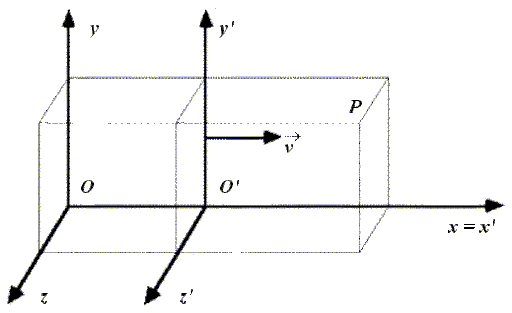
\includegraphics[width=0.45\linewidth]{Immagini/MTTR.png}
    \caption{un sistema fisso $O$ e un sistema mobile $O'$ in moto di trascinamento traslatorio rettilineo lungo l'asse $x$.}
    \label{fig: MTTR}
\end{figure}
Nel primo caso, le relazioni per la velocità e l'accelerazione sono 
\begin{equation}
    \vv=\vvi+\vv_{O'},\quad\va=\vai,
\end{equation}
mentre il legame tra i raggi vettori è 
\begin{equation}
    \vr=\vr_{O'}+\vri=\vv_{O'}t+\vri,
\end{equation}
infatti $\vr_{O'}=\vv_{O'}t$ nell'ulteriore ipotesi che per $t=0$ le origini coincidano. Le relazioni vettoriali possono essere proiettate sugli assi cartesiani fornendo le relazioni tra le componenti dei vettori. Le relazioni che si ottengono prendono il nome di trasformazione galileiane e sono
\begin{equation}
\label{eq: trasformazioni di Galileo}
    \begin{cases}
        x'=x-v_{O'}t \\
        v_x'=v_x-v_{O'} \\
        a_x'=a_x
    \end{cases},\quad
    \begin{cases}
        y'=y \\
        v_y'=v_y \\
        a_y'=a_y
    \end{cases},\quad
    \begin{cases}
        z'=z \\
        v_z'=v_z \\
        a_z'=z_z
    \end{cases}.
\end{equation}
Nel secondo caso, supponendo che $O'$ abbia un'accelerazione costante $\va_{O'}=\va_t$ e una velocità iniziale $\vv_{i}$, ambedue parallele e concordi all'asse $x\equiv x'$. Quindi, la posizione e la velocità $O'$ sono espresse da
\begin{equation}
    x_{O'}=v_it+\frac{1}{2}a_tt^2,\quad v_{O'}=v_i+a_tt,
\end{equation}
e le relazioni per la velocità e l'accelerazione sono
\begin{equation}
    \vv=\vvi+\vv_{O'},\quad\va=\vai+\va_{O'}.
\end{equation}
Dunque, le relazioni \eqref{eq: trasformazioni di Galileo} diventano
\begin{equation}
    \begin{cases}
        x'=x-v_it-\dfrac{1}{2}a_tt^2 \\
        v_x'=v_x-v_i-a_tt \\
        a_x'=a_x-a_t
    \end{cases},\quad
    \begin{cases}
        y'=y \\
        v_y'=v_y \\
        a_y'=a_y
    \end{cases},\quad
    \begin{cases}
        z'=z \\
        v_z'=v_z \\
        a_z'=z_z
    \end{cases}.
\end{equation}

\section{Moto di trascinamento rotatorio uniforme}
Si consideri la situazione mostrata in figura \ref{fig: MTRU}. In questo caso si ha che $\vr=\vri$ (origini coincidenti), $\vv_{O'}=0$, $\va_{O'}=0$, $\vom=costante$ e le relazioni per la velocità e l'accelerazione sono
\begin{equation}
    \vv=\vvi+\vom\times\vr,\quad\va=\vai+\vom\times(\vom\times\vr)+2\vom\times\vvi.
\end{equation}
Quindi, l'equazione \eqref{eq: forza in un SdRNI} diventa
\begin{equation}
    \vF+\vF_{centr}+\vF_{Cor}=m\vai,
\end{equation}
dove $\vF_{centr}=-m\vom\times(\vom\times\vr)$ è la forza centrifuga e $\vF_{Cor}=-2\vom\times\vvi$ è la forza di Coriolis, le quali hanno lo stesso ruolo della forza $-m\va_t$ visto in precedenza.  
\begin{figure}[h]
    \centering
    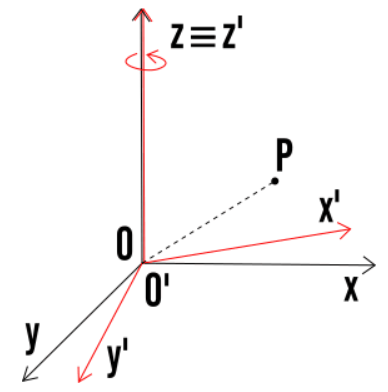
\includegraphics[width=0.3\linewidth]{Immagini/MTRU.png}
    \caption{un sistema fisso $O$ e un sistema mobile $O'$ in moto di trascinamento rotatorio uniforme.}
    \label{fig: MTRU}
\end{figure}
\begin{ex}
    Si consideri un filo a piombo su una piattaforma orizzontale ruotante attorno ad un asse con il punto di sospensione fuori dall'asse di rotazione. Il filo si inclina di un angolo $\theta$ rispetto alla verticale crescente con $\vom$ e con la distanza $r$ dall'asse di rotazione. Il corpo puntiforme non si muove rispetto alla piattaforma, quindi $\vvi=0$ e $\vF_{Cor}=0$.
    \begin{figure}[H]
        \centering
        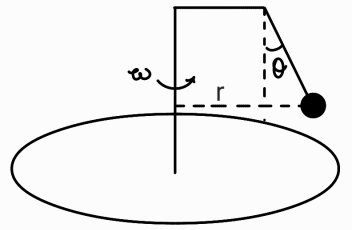
\includegraphics[width=0.37\linewidth]{Immagini/pendolo relativo.png}
        \caption{filo a piombo ruotante.}
        \label{fig: filo a piombo ruotante}
    \end{figure}
    
    Per un osservatore inerziale, il moto di rotazione del corpo è determinato dalle forze vere, ovvero dalla forza peso $m\vg$ e dalla tensione del filo $\vT$. Quindi
    \begin{equation}
        \vT+m\vg=m\va=m\omega^2r\hatu_r.
    \end{equation}
    Dalla figura \ref{fig: filo a piombo ruotante}, si hanno
    \begin{equation}
        T\sin{\theta}=m\omega^2r,\quad T\cos{\theta}=mg,\quad \tan{\theta}=\frac{a}{g}=\frac{\omega^2r}{g}.
    \end{equation}
    La forza centripeta richiesta per mantenere in rotazione il corpo su una circonferenza di raggio $r$ è fornita dalla componente orizzontale della tensione. 
    
    Invece, per un osservatore solidale alla piattaforma il corpo puntiforme è fermo, per cui 
    \begin{equation}
        \vT+m\vg+\vF_{centr}=0\Rightarrow\vF_{centr}=m\omega^2r\hatu_r.
    \end{equation}
    Le forze sono equilibrate dalla forza centrifuga apparente. In ogni caso, misurato $\theta$ è possibile calcolare l'accelerazione centrifuga, ovvero l'accelerazione con cui ruota il sistema non inerziale, usando $\tan{\theta}=\omega^2r/g$.
\end{ex}